\chapter{Estado de la Cuestión}
\label{cap:estadoDeLaCuestion}
En este capítulo se hará una investigación sobre las técnicas, herramientas y formas de crear inteligencias artificiales para enemigos.
Para ello vamos a comenzar haciendo un recorrido por elementos generales relacionados con la inteligencia artificial y cómo se usan en videojuegos de plataformas en 2D, ya sea para crear Non-Player Characters (NPC) o enemigos.
Se mencionarán además herramientas para conseguir los fines descritos anteriormente y se hablará de algunos motores de videojuegos que han inspirado algunos aspectos de nuestra herramienta. \\


\section{Introducción a la Inteligencia Artificial en videojuegos}

La Inteligencia Artificial (IA) en videojuegos se refiere a los algoritmos de toma de decisiones que controlan el comportamiento de los personajes dentro del juego, según lo define Bakkes en su tesis doctoral \cite{Bakkes2010}.\\

La IA desempeña un papel crucial, especialmente en entornos 2D donde la utilidad en los enemigos es lo que determina en mayor medida el nivel de dificultad y la jugabilidad del videjuego. Desde los inicios donde se  presentaban enemigos con comportamientos simples facilmente memorizable por los usuarios hasta la actualidad más compleja que logra enemigos “más humanos” y mejora la inmersión. El potencial de la IA y la razón por la que suscita tanto interés, radica en su capacidad de actuar de forma autónoma: no se limita a seguir instrucciones predefinidas, sino que es capaz de tomar decisiones adaptativas en función del contexto.\\

Por ejemplo, la IA puede adaptarse dinámicamente a las decisiones del jugador, como ocurre con el enemigo principal en  \cite{Hope2014}, donde el comportamiento del Alien se ajusta de forma impredecible para mantener la tensión. También puede utilizarse para generar contenido procedural, como en juegos roguelike tipo \textit{Hades}\footnote{\url{https://hades.fandom.com/es/wiki/Hades_(juego)}}, o para entrenar agentes mediante redes neuronales profundas que imitan el estilo de conducción de jugadores humanos, como sucede en la saga \textit{Forza Motorsport}\footnote{\url{https://forza.fandom.com/wiki/Forza_Wiki}}.\\

En definitiva, el uso de la IA en videojuegos responde a una necesidad técnica y creativa: la de crear experiencias de juego más inmersivas, adaptativas, eficientes y realistas. Tal como se expone en \cite{YannakakisTogelius2018}, la IA no solo permite que el juego ``juegue bien'', sino que también posibilita que lo haga de forma convincente y útil para diseñadores y jugadores por igual.


\section{Técnicas de toma de decisiones en NPC`s}
Existen muchas técnicas que se pueden abordar a la hora de modelar una IA. Para decidir cuál se ajusta mejor a un problema en concreto, es importante saber ciertos factores, como por ejemplo la complejidad esperada del comportamiento, la adaptabilidad y flexibilidad de la técnica, si queremos invertir mucho tiempo en implementar estas técnicas o queremos algo rápido de hacer y funcional o los recursos que consumen. \\
A continuación, se presentan técnicas utilizadas en videojuegos para modelar IA, las cuales hemos seleccionado porque comparten una estructura similar a la que planteamos inicialmente. Entre ellas, las maquinas finitas de estados se ajustan especialmente a nuestro enfoque y serán las que utilizaremos en nuestro desarrollo.

\subsection{Máquinas de estado finitas}
En su obra, \cite{MillingtonFunge2016} describen las máquinas de estado finitas(FSM) como una de las herramientas más comunes y efectivas para construir IA en videojuegos. Una FSM se compone de un conjunto finito de estados, donde solo uno está activo en un momento dado, y cada estado contiene un comportamiento asociado así como reglas que determinan las transiciones a otros estados en función de eventos o condiciones.\\
En el contexto de los videojuegos, las FSM permiten definir con claridad cómo debe comportarse una entidad del juego en distintas situaciones, por ejemplo: caminando, atacando, huyendo o patrullando. La estructura garantiza que solo un estado esté activo a la vez, lo que simplifica la lógica de control y evita conflictos entre comportamientos simultáneos. 
A menudo, una FSM se representa como un grafo, donde los nodos representan los estados, que realizan las acciones y las aristas las transiciones posibles, activadas por eventos o condiciones del entorno. Esta estructura modular y determinista facilita tanto su diseño como su implementación y depuración.\\

Como se documenta en el artículo de Gopalakrishnan y Pradeep \cite{Gopalakrishnan2021}, el primer videojuego documentado que utilizó FSM para implementar la lógica de juego fue \textit{Spacewar!(1961)} desarrollado en el MIT por Steve Russell. Este videojuego implementaba una lógica basada en estados para manejar el comportamiento de las naves, la detección de colisiones y la física del juego. Aunque no usaba una implementación formal de máquinas de estado, sí modelaba cambios entre estados bien definidos, como el movimiento de las naves o la activación de los disparos. \\ 

\textit{Pac-Man}\footnote{\url{https://pacman.fandom.com/es/wiki/Pac-Man_Wiki:Portada}} es un videojuego que usa FSM, en el que el jugador controla un personaje amarillo en forma de círculo con una boca que se abre y cierra constantemente. Fue lanzado en 1980 por la compañía japonesa Namco (actual Bandai Namco). El objetivo de este videojuego es recorrer un laberinto e ir comiendo todos los puntos mientras evitamos cuatro fantasmas hasta que comemos una píldora de poder que nos hace invulnerable y nos da la capacidad de comer a los fantasmas. Estos huirán tras comernos la píldora.\\
La complejidad en la IA de Pac-Man es asombrosa porque se le quiso dar profundidad al juego haciendo que cada fantasma tuviera una personalidad diferente. Para ello se implementó una máquina de estado por fantasma haciendo que la forma en la que interactúan con el entorno sea ligeramente diferente.
\begin{figure}[t]
	\centering
	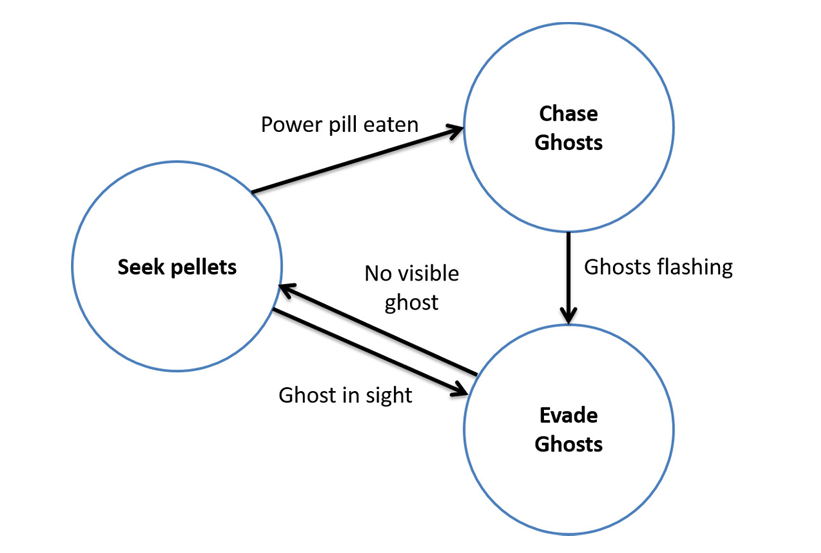
\includegraphics[height=5cm]{Imagenes/FMS_MsPac-man.png}
	\caption{Comportamiento del jugador en \textit{Pac-Man}, basado en una máquina de estados finita, extraído de \cite{YannakakisTogelius2018}.}
	\label{fig:Comportamiento jugador Pac-Man}
\end{figure}
A continuación se enumerarán los fantasmas y sus formas de comportarse.
\begin{itemize}
	 \item Blinky: es el fantasma rojo y su papel es el de cazador, siendo su personalidad la más agresiva, hecho que se refleja en que es el único fantasma que comienza fuera de la casa de los fantasmas y que tras salir empieza a perseguir al jugador incansáblemente. Tiene otra característica propia, a medida que el jugador va comiendo bolitas, comienza a aumentar su velocidad.
	 \item Pinky: como su nombre indica es el fantasma de color rosa. En japonés se llama \textit Machibuse, el que tiende emboscadas. Pinky es el interceptor del juego por lo que va a tratar de cortar el camino del jugador. Es un fantasma relativamente rápido, por lo que calculará constantemente hacia donde se dirige el jugador para usar su velocidad para adelantarse y cortar el paso.
	 \item Inky: el fantasma azul es el más impredecible de todos, deambula tranquilo por el laberinto hasta que está cerca del jugador y entonces, lo persigue.
	 \item Clyde: el fantasma naranja y el más tranquilo de todos. Suele ser el último en salir de la casa de los fantasmas y no intentará atrapar al jugador en ningún caso. 
\end{itemize}
Para ilustrar el funcionamiento del juego se usará la Figura \ref{fig:Comportamiento jugador Pac-Man} que representa una posible FSM para el jugador, lo que haría que las decisiones tomadas fueran lo más eficientes posibles en el momento.\\


\subsubsection{Máquinas de estado finitas jerárquicas}
La principal desventaja de las FSM es que son muy inflexibles y estáticas y, aunque se puede atenuar mediante la implementación de probabilidades o reglas que no estén tan claras a la hora de hacer las transiciones, siguen aunmentando su complegidad progresivamente cuando aumenta su tamaño. Una  forma de poder simplificar esa complegidad es sub-dividiendo tareas complejas en otras más sencillas. Permitiendo agrupar varias máquinas finitas dentro de una otra máquina finita. Las Maquinas de estado jerárquicas (HFSM) tienen la misma representación que las FSM, diferenciandose por la representación anidada de estados dentro de otros estados \cite{JorgeHFSM}.
\begin{figure}[h!]
	\centering
	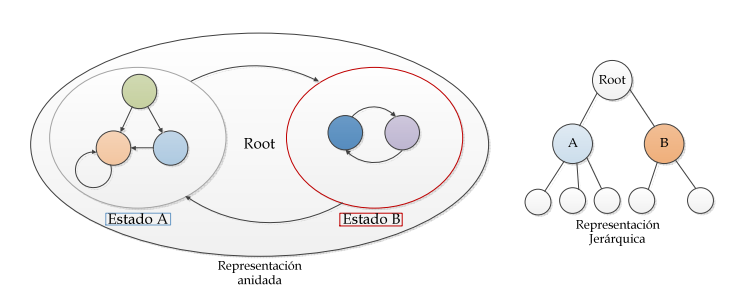
\includegraphics[height=5cm]{Imagenes/HFSM.png}
	\caption{Ejemplo de maquinas de estado jerárquicas extraido de \cite{JorgeHFSM}.}
	\label{fig:Maquinas de estado jerárquicas}
\end{figure}

\subsection{Árboles de comportamiento}

Un Árbol de Comportamiento (Behavior Tree o BT) es una técnica utilizada para modelar la toma de decisiones en inteligencia artificial, especialmente en videojuegos. Es conceptualmente similar a una Máquina de Estados Finitos, ya que también organiza el comportamiento en unidades que se activan de forma exclusiva (es decir, solo una parte del árbol está ``activa'' en cada momento). Sin embargo, en lugar de representar estados, los BT están formados por nodos que representan comportamientos, organizados jerárquicamente en forma de árbol. Cada nodo ejecuta una acción o toma una decisión, y el control fluye a través del árbol según unas reglas predefinidas. \\

Los nodos de un BT pueden dividirse en varias categorías, siendo las principales:

\begin{itemize}
\item Nodos hoja (leaf nodes): Acciones concretas que ejecuta el agente, como moverse a un punto'' o ``atacar al enemigo''.
\item Nodos compuestos: Agrupan varios nodos hijos y determinan en qué orden deben ejecutarse (por ejemplo, secuencias o selectores).
\item Nodos de control o decoradores: Modifican el comportamiento de los nodos hijos (por ejemplo, repetir un nodo mientras se cumpla una condición).
\end{itemize}

La principal ventaja respecto a las Máquinas de Estado Finitas es su modularidad, la capacidad que tiene un sistema de dividir la lógica del comportamiento en piezas independientes y reutilizables, pudiendo agrupar estas piezas en grupos que a su vez funcionan como una pieza. Su facilidad para ser diseñados y probados han hecho que los árboles de comportamiento se conviertan en una opción real para modelar IA en la industria del videojuego, con juegos como \textit{Bioshock} \citep{bioshock} y \textit{Halo 2} \citep{halo2} como referencias en el uso de Árboles de comportamiento.\\

Un ejemplo no tan conocido de uso de Árboles de comportamiento en la industria del videojuego es \textit{Spore} \citep{spore}. \textit{Spore} es un videojuego en el que el jugador va a comenzar creando una célula y va encarnarla durante todo el proceso de su evolución hasta que esta se convierta en un ser mucho más complejo llegando incluso a construir una civilización muy avanzada. La inteligencia artificial de las entidades que nos rodean en este videojuego están fundamentadas en Árboles de comportamiento.\\

La gran diferencia en cómo Spore utiliza los Árboles de Comportamiento frente a juegos como Halo 2 es que separa el concepto de decider del de behavior. En Halo 2, los árboles están compuestos por behaviors (comportamientos que pueden ser grupales o individuales) y impulsos (transiciones entre comportamientos basadas en prioridades). Esta estructura, aunque funcional, tiende a generar problemas de escalabilidad, como:
\begin{itemize}
	\item Dificultad para entender y mantener el árbol.
	\item Duplicación innecesaria de comportamientos.
	\item Poca reutilización del código.
	\item Aumento del riesgo de errores al introducir nuevas acciones o decisiones.
\end{itemize}

Para resolver estos problemas, el equipo de Maxis decidió separar completamente los nodos de decisión (deciders) de los nodos de acción (behaviors). Los deciders actúan como controladores que eligen qué behavior ejecutar en función del contexto, mientras que los behaviors se mantienen como bloques de acción reutilizables. Esta estructura modular y jerárquica no solo mejora la claridad del árbol, sino que también facilita su escalabilidad y mantenimiento en proyectos complejos como Spore.\\

La Figura \ref{fig:BT Spore} es un ejemplo de un BT sacado de las documentación\footnote{ \url{https://chrishecker.com/My_Liner_Notes_for_Spore/Spore_Behavior_Tree_Docs}} que hay publicada del juego.
En este árbol, los nodos se dividen en dos tipos principales:
\begin{itemize}
\item Nodos de decisión (deciders): Representados con forma de rombo (como \textit{GUARD}, \textit{EAT}, \textit{IDLE}), son los encargados de seleccionar cuál de sus nodos hijos ejecutar en función del contexto o condiciones actuales. Evalúan a sus hijos en orden y seleccionan el primero que sea válido.
\item Nodos de acción (behaviors): Representados con rectángulos (como \textit{FIGHT}, \textit{PATROL}, \textit{YELL\_FOR\_HELP}), son los encargados de ejecutar una acción concreta dentro del mundo del juego. Estas acciones son atómicas y no contienen lógica de decisión propia.
\end{itemize}

El nodo raíz (\textit{ROOT}) inicia la ejecución del árbol. El flujo de control comienza en este nodo y se propaga hacia abajo evaluando nodos hijos de izquierda a derecha. Cuando un decider es activado, se encarga de decidir cuál de sus hijos (otros deciders o behaviors) debe activarse en ese momento. Si ninguno de los hijos es adecuado, se retorna al nodo anterior, lo que permite reconsiderar otras opciones disponibles. Este enfoque permite que el comportamiento sea flexible y jerárquico.

Gracias a esta organización, se logra modularidad y escalabilidad: por ejemplo, el decider \textit{IDLE} encapsula comportamientos distintos como \textit{REST} o \textit{PLAY}, y este último a su vez contiene subacciones como \textit{FLIP}, \textit{ROLL} o \textit{DANCE}. Esta jerarquía hace posible reutilizar comportamientos en distintos contextos y facilita el mantenimiento del árbol.

\begin{figure}[t]
	\centering
	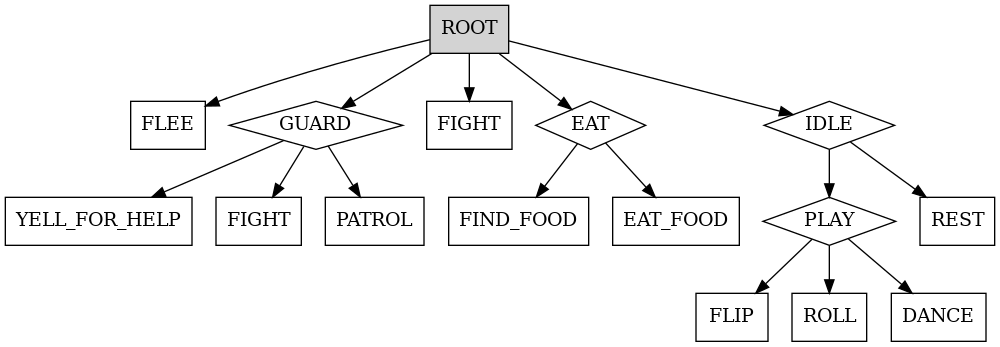
\includegraphics[width = 0.7\textwidth]{Imagenes/BT_Spoore.png}
	\caption{Ejemplo BT, Documentación Spore}
	\label{fig:BT Spore}
\end{figure}
\subsection{Goal-Oriented Action Planning}

GOAP es un sistema basado en planificación de acciones. En lugar de definir comportamientos fijos como hemos visto anteriormente, la entidad analiza la situación y construye un plan para alcanzar el objetivo designado.
Esta técnica fue desarrollado en el \textit{MIT} por \textit{\citet{GOAP_Jeff_Orkin}} a principio de siglo. \\

La entidad pasa a ser un agente autónomo que tiene la capacidad de planificar de manera dinámica una secuencia de acciones para satisfacer una meta. Para llegar a esa meta se tendrán en cuenta el contexto del agente, por lo que dependiendo de este se podrá llegar a la meta de varias maneras, aunque la utilizada será la mejor valorada, de esta manera se reduce lo repetitivo que pueda llegar a ser lidiar con un tipo de agente, ya que siendo el enemigo, por ejemplo, este abordará al jugador de manera distinta dependiendo de la situación en la que se encuentre.\\

El enfoque de GOAP es muy parecido a una Máquina de Estado Finita, pero en GOAP las acciones y metas no van de la mano, sino que se separan para abrir la posibilidad de tener un proceso de planificación dinámico y adaptativo.
La escalabilidad que ofrece GOAP es mayor a todas las técnicas vistas anteriormente.\\

El considerado primer videojuego que usa GOAP es \textit{F.E.A.R, Monolith Productions}\footnote{\url{https://www.gdcvault.com/play/1013282/Three-States-and-a-Plan}}. El propio Jeff Orkin explica que en el videojuego se quería llegar a una complejidad en la IA a la que las Máquinas de Estado Finitas no podían llegar, por lo que optaron por no excluirlas pero solo tener tres estados y usar un algoritmo \textit{A*} para planear las acciones a realizar. Un ejemplo es que si el jugador cierra una puerta mientras es perseguido por un enemigo, el enemigo puede dinámicamente volver a rehacer su plan y decidir si buscar un hueco para disparar, por ejemplo una ventana, o buscar una entrada alternativa. Esta libertad en las acciones de los agentes liberan a los desarrolladores para que estos puedan enfocarse en el manejo de grupos, como fuego de supresión, cobertura y búsqueda del jugador.\\

A continuación vamos a definir una serie de términos clave para definir el comportamiento de GOAP.
\begin{itemize}
	 \item Objetivos: Lo que la entidad quiera lograr. Un agente puede querer cumplir más de un objetivo. En el videojuego \textit{NOLF 2}, como se menciona en \citet{GOAP_Jeff_Orkin}, los personajes tenían típicamente alrededor de 25 objetivos, aunque en cada instante solo un objetivo esté activo y este determine las acciones del agente. Un objetivo sabe como calcular su relevancia actual y sabe cuando ha sido alcanzado.\\
Aunque conceptualmente son similares, hay una diferencia clave entre los objetivos en \textit{NOLF 2} y GOAP y es que en el primero cada objetivo tiene un plan predefinido con pasos fijos y ramas condicionales establecidas de antemano y en GOAP los objetivos solo definen las condiciones que deben cumplirse para darse por terminado, los pasos para alcanzarlos se generan dinámicamente en tiempo real.

	 \item Plan: Forma de denominar una secuencia de acciones. Un plan válido es aquel que lleva a un personaje desde un estado inicial hasta un estado que cumple con el objetivo. El plan se ejecuta hasta que se complete, se invalide u otro objetivo se vuelva más importante lo que obligará a que se cree formule un nuevo plan.

	 \item Acción: Una acción es un paso único y atómico dentro de un plan que hace que un personaje haga algo. Algunas acciones posibles en \textit{NOLF 2} es \textit{Go To Point}, \textit{Draw Weapon}...
La duración de una acción puede variar, por ejemplo la acción \textit{Reload Weapon} terminará cuando la acción acabe, mientras que la acción \textit{Attack} puede continuar indefinidamente hasta que el objetivo muera.\\
Cada acción determina cuándo puede ejecutarse y qué impacto tendrá en el mundo del juego, es decir una acción conoce sus \textit{precondiciones} y sus \textit{efectos}.
	
	\item Mundo: Estado actual del contexto de la entidad.
 	
	\item Planificador: Encuentra la secuencia de acciones para lograr el objetivo partiendo del estado actual del agente. Si tiene éxito devolverá un plan que el personaje seguirá para guiar su comportamiento.\\

Para ilustrar el funcionamiento del planificador usaremos la Figura \ref{fig:GOAP_Planificador}.
Los rectángulos representan el estado inicial y el estado objetivo, los círculos representan las acciones disponibles.
En este caso, el objetivo es matar a un enemigo, por lo que el estado final es aquel en el que el enemigo está muerto, en otras palabras, el planificador tiene que encontrar una secuencia de acciones que tome al mundo desde un estado en el que el enemigo está vivo hasta otro en el que este está muerto.\\
Este proceso se aborda como un \textit{pathfinding}, la búsqueda de un camino válido que nos lleve desde el estado inicial al estado final. El planificador tiene que encontrar un plan válido y no siempre este es el esperado por el usuario. 


\begin{figure}[t]
	\centering
	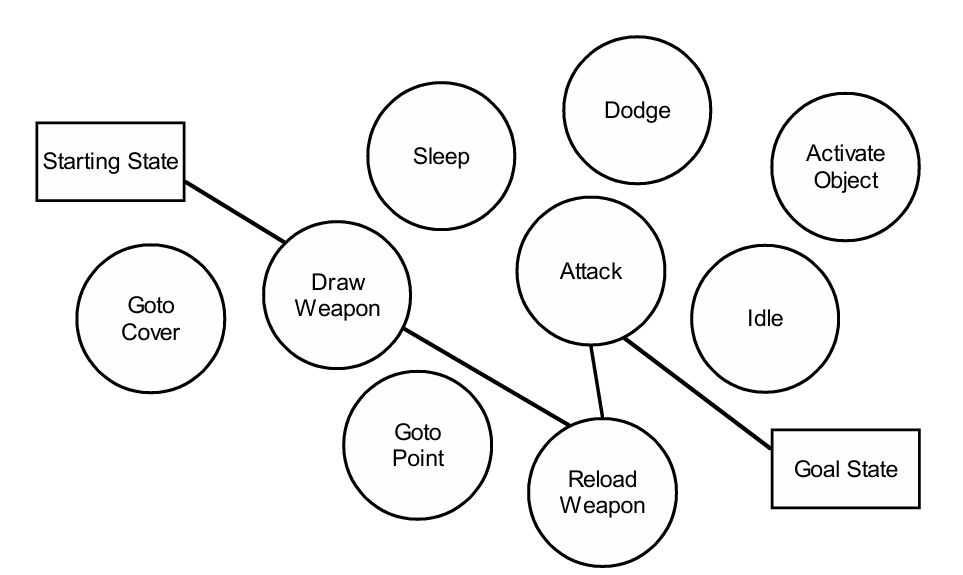
\includegraphics[width = 0.7\textwidth]{Imagenes/GOAP_Planificador.png}
	\caption{Ejemplo ilustrativo de GOAP donde el estado final es la eliminación de un enemigo.}
	\label{fig:GOAP_Planificador}
\end{figure}
	
	
\end{itemize}
\comp{https://github.com/crashkonijn/GOAP herramienta que podriamos analizar}\\ 
\section{Análisis de herramientas para la creación de comportamientos inteligentes}

Tras abordar técnicas usadas para la toma de decisiones, se ha visto que en ocasiones la complejidad de crear esos algoritmos no es del todo trivial. Por ello, surge la necesidad de crear herramientas que ayudasen a los desarrolladores a crear Inteligencias Artificiales de toma de decisiones, concretamente cenrada en la creación de NPCs. Teniendo en cuenta que la creación de IA debe estar al alcance de personas con nulo conocimiento de programación, estas herramientas deben implementar una interfaz gráfica para que el funcionamiento de la IA sea más visual.
A continuación, se han seleccionado algunas herramientas que ayudan a dicha creación como ejemplo.\\

\subsection{Behavior Bricks}

\textit{Behavior Bricks}\footnote{\url{https://bb.padaonegames.com/doku.php}} es una herramienta disponible para el motor de videojuegos \textit{Unity} centrada en cubrir todas las necesidades de implementación de comportamientos para juegos. Con \textit{Behavior Bricks} el usuario es capaz de modelar de manera visual tanto Máquinas de Estado Finitas como Árboles de comportamiento.\\
\begin{figure}[t]
	\centering
	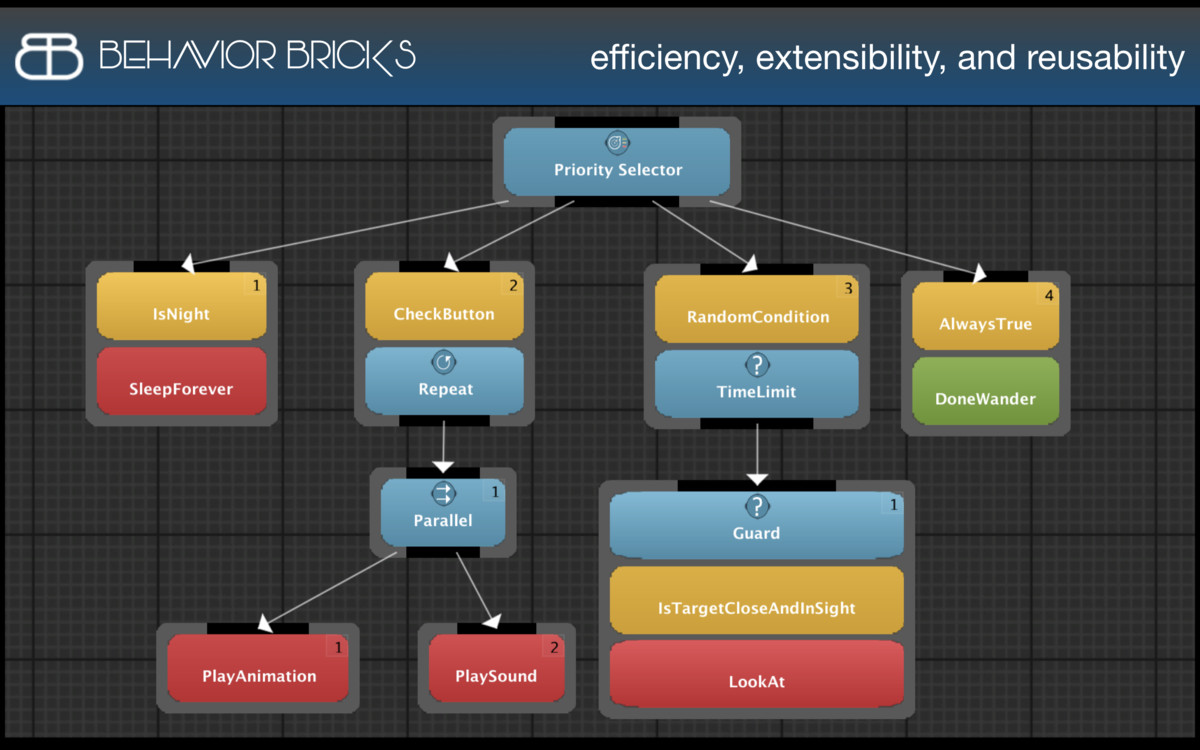
\includegraphics[width = 0.7\textwidth]{Imagenes/Behavior_Bricks.jpg}
	\caption{Ejemplo de uso de Behavior Bricks}
	\label{fig:BH_Figure}
\end{figure}

\textit{Behavior Bricks} es una herramienta de scripting visual, por lo que favorece una colaboración entre diseñadores y programadores un aspecto que frecuentemente plantea desafíos.\\
Otra particularidad de \textit{Behavior Bricks} es su modularidad, ya que permite modificar cada una de las partes con muy poco acoplamiento entre ellas, lo que incita a su reutilización en distintos proyectos. Esta modularidad también permite que podamos tener un estado/comportamiento que sea en sí mismo un grupo de estados/comportamientos.\\
Esta herramienta hace hincapié en no ralentizar significativamente el rendimiento del juego, gracias a su optimización y la gestión de memoria la cual a veces es compartida entre estados/comportamientos para ahorrar recursos.\\

\subsection{PlayMaker}
PlayMaker\footnote{\url{https://hutonggames.com/}} es un editor visual de FSM para Unity diseñado especialmente para artistas y diseñadores, ya que permite desarrollar IA sin necesidad de escribir código.

Su interfaz es altamente visual e intuitiva. Al crear una FSM, se genera automáticamente un estado inicial llamado \textit{START}, como podemos ver en la Figura \ref{fig:PlayMaker_Figure}, seguido de un estado predeterminado llamado \textit{State 1}, al cual se transiciona al ejecutar \textit{Unity}. A partir de ahí, el usuario puede agregar más estados y definir eventos que permiten cambiar entre ellos según ciertas condiciones.

Una de sus principales ventajas es la facilidad con la que se pueden modificar los valores de los componentes de \textit{Unity}. Basta con arrastrar un componente a la pestaña \textit{State} para ajustar sus propiedades dentro de un estado determinado. Además, PlayMaker proporciona una amplia colección de acciones predefinidas, como la detección de entrada de teclas, temporizadores y movimientos entre otros. Estas acciones pueden activar eventos que actúan como transiciones entre estados, facilitando la creación de mecánicas de juego complejas sin necesidad de programación.

Gracias a su flexibilidad y facilidad de uso, PlayMaker es ideal para diseñar IA, lógica de juego, animaciones, interacción con interfaces de usuario y prototipos rápidos, convirtiéndolo en una herramienta poderosa tanto para principiantes como para desarrolladores experimentados que buscan agilizar su flujo de trabajo. Otro punto fuerte de PlayMaker es que permite que la herramienta sea escalable con scripts propios.

PlayMaker está disponible en la \textit{asset store} de \textit{Unity}, aunque su precio hace que desarrolladores con pocos recursos tengan que descartar esta opción, no deja de ser una herramienta usada ampliamente por la comunidad de desarrolladores, habiendo sido utilizada en juegos como el aclamado por la crítica \textit{Hollow Night}\footnote{\url{https://hollowknight.fandom.com/wiki/Hollow_Knight_Wiki}}, \textit{Firewatch}\footnote{\url{https://www.firewatchgame.com/}} la aventura narrativa del estudio norteamericano Campo Santo o el juego de plataforma de los creadores de \textit{Limbo}, \textit{INSIDE}\footnote{\url{https://inside.fandom.com/wiki/Inside_Wiki}}.\\

\begin{figure}[t]
	\centering
	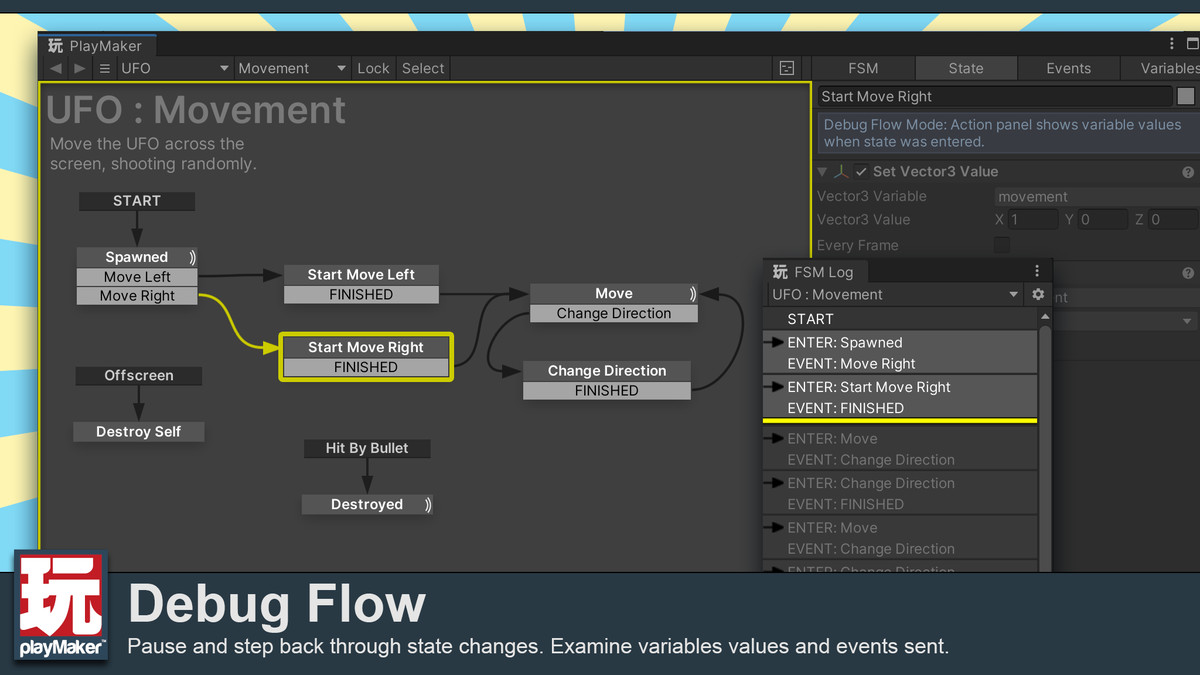
\includegraphics[width = 0.7\textwidth]{Imagenes/PlayMaker.jpg}
	\caption{Ejemplo de uso de Play Maker}
	\label{fig:PlayMaker_Figure}
\end{figure}
\subsection{Decisión}
Tras el análisis de las herramientas con capacidad para integrar comportamientos de inteligencia artificial, surgieron opciones relevantes que nos permiten la integración con Unity. Si bien esas herramientas son completamente válidas, se ha optado por la creación de una herramienta propia, partiendo desde cero. Esta decisión se fundamenta en la necesidad de personalización y control exhaustivo. Superando así las posibles limitaciones económicas de la investigación y las posibles faltas de adecuación total con otras herramientas.
\section{Motores de videojuegos}

La siguiente sección consistirá en el análisis de distintos motores de videojuegos. El objetivo  de este análisis es proporcionar una comprensión sobre cuales son las fortalezas y debilidades de cada uno de ellos, para así, razonar justificadamente cual se ajustamás a las necesidades de estre proyecto. Todos los motores escogidos tienen gran renombre en la industria ofreciendo gran variedad y distintas filosofías de diseño.
\subsection{Unity}
\textit{Unity}\footnote{\url{https://unity.com}} es un motor de videojuegos desarrollado por \textit{Unity Technologies} que se ha convertido en una de las herramientas más utilizadas en la industria del desarrollo de videojuegos. Su versatilidad y facilidad de uso han permitido la creación de títulos de gran éxito como \textit{Hollow Knight}\footnote{\url{https://www.hollowknight.com}}, \textit{Cuphead}\footnote{\url{https://cupheadgame.com}} y \textit{Genshin Impact}\footnote{\url{https://genshin.hoyoverse.com/es}}. La versión más actual del motor, \textit{Unity 6.0}, incorpora mejoras en su sistema de renderizado, herramientas avanzadas de optimización y un motor de físicas más eficiente.\\

Uno de los aspectos más destacados de \textit{Unity} es su capacidad para desarrollar videojuegos tanto en 2D como en 3D, lo que lo convierte en una opción ideal para una amplia variedad de proyectos. El motor ofrece dos principales opciones para la programación: el lenguaje \textit{C\#}, utilizado para la creación de scripts avanzados, y el sistema visual \textit{Bolt}, que permite desarrollar lógica de juego sin necesidad de escribir código.\\

El sistema de scripting en \textit{Unity} está basado en \textit{C\#} y funciona a través del uso de \textit{MonoBehaviour}, una clase base que permite definir el comportamiento de los objetos del juego. Los scripts, son usados para implementar componentes. Estos componentes se adjuntan a los objetos (gamebjects) dentro del editor (Figura \ref{fig:Unity_Inspector}) y pueden controlar aspectos como la física, la inteligencia artificial y las interacciones del jugador.\\

\begin{figure}[t]
	\centering
	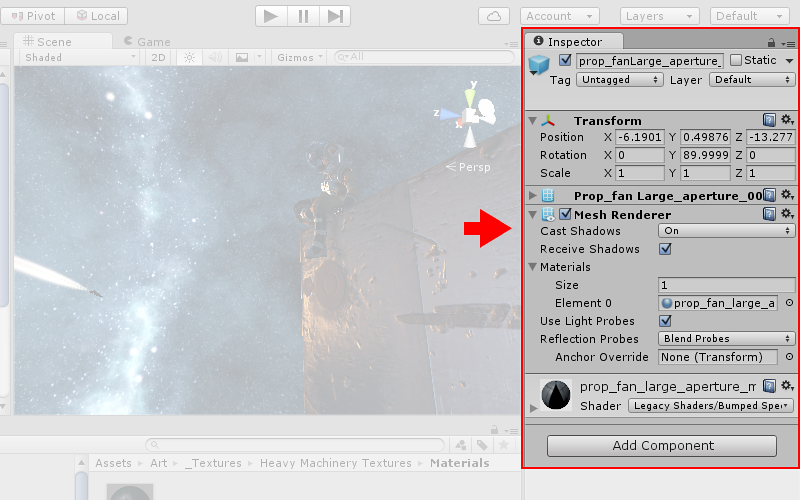
\includegraphics[width = 0.7\textwidth]{Imagenes/InspectorWindowCallout.png}
	\caption{Inspector de Unity, con una serie de componentes}
	\label{fig:Unity_Inspector}
\end{figure}

Por otro lado, el sistema de programación visual \textit{Bolt}\footnote{\url{https://docs.unity3d.com/2019.3/Documentation/Manual/VisualScripting.html}} permite a los desarrolladores sin experiencia en programación crear juegos mediante una interfaz basada en nodos, este sistema permite definir lógica de juego conectando bloques de funciones y eventos sin necesidad de escribir una sola línea de código.\\

Además de su versatilidad en la programación, \textit{Unity} cuenta con un conjunto de herramientas avanzadas para la creación de entornos, animaciones y físicas. Su sistema de renderizado \textit{Universal Render Pipeline (URP)} permite optimizar los gráficos para múltiples plataformas, mientras que el \textit{High Definition Render Pipeline (HDRP)} está diseñado para juegos con gráficos de alta calidad en PC y consolas de última generación.\\

Si se compara con otros motores como \textit{Unreal Engine}, del cual se hablará más adelante, \textit{Unity} destaca por su flexibilidad y menor consumo de recursos. Mientras que \textit{Unreal Engine} es ampliamente reconocido por su calidad gráfica superior, \textit{Unity} ofrece un entorno más ligero y optimizado, lo que lo convierte en una mejor opción para desarrolladores independientes o proyectos móviles. Sin embargo, su sistema visual de nodos es menos avanzado que el de \textit{Unreal}, lo que puede requerir el uso de \textit{C\#} para acceder a funcionalidades más complejas.\\

Un punto negativo de \textit{Unity} con respecto a otros motores es su modelo de licencias y sus cambios recientes en la política de precios, lo que ha generado controversia entre los desarrolladores. A pesar de esto, su comunidad activa, su gran cantidad de recursos educativos y su compatibilidad con una amplia variedad de plataformas lo mantienen como una de las opciones más accesibles y populares para la creación de videojuegos.

La combinación de herramientas avanzadas y la facilidad de uso hace que cualquier persona pueda desarrollar desde juegos móviles y experiencias en realidad virtual hasta títulos en 3D de gran escala sin necesidad de contar con un equipo grande o conocimientos avanzados de programación.

\subsection{Unreal Engine}
\textit{Unreal Engine}\footnote{\url{https://www.unrealengine.com/es-ES}}, desarrollado por \textit{Epic Games}\footnote{\url{https://www.epicgames.com/site/es-ES/home}}, es uno de los motores de videojuegos más potentes y utilizados en la industria de los videojuegos en títulos como la saga \textit{Hellblade}\footnote{\url{https://thehellblade.fandom.com/wiki/Hellblade:_Senua\%27s_Sacrifice}} o el éxito mundial \textit{Fornite}\footnote{\url{https://www.fortnite.com/?lang=es-ES}} y la versión más actual es Unreal Engine 5 que cuenta, entre otras cosas, con \textit{Lumen}, un sistema de iluminación global dinámica o la mejora sustancial del sistema de simulación de físicas \textit{Chaos}.\\
A pesar de que permite la programación en \textit{C++}, también ofrece un sistema visual llamado Blueprints, diseñado para que cualquier persona, sin conocimientos de programación, pueda crear videojuegos completos mediante una interfaz gráfica intuitiva.

El sistema de Blueprints funciona de manera similar a un lenguaje de programación visual basado en nodos. En lugar de escribir código manualmente, el usuario conecta bloques de lógica (Figura \ref{fig:BluePrints_Figure}) para definir comportamientos, interacciones y mecánicas dentro del juego. Esto permite crear desde movimientos de personajes y mecánicas de combate hasta sistemas complejos de inteligencia artificial y físicas sin necesidad de escribir una sola línea de código. Cabe destacar que se pueden crear Blueprints en caso de que sea necesario.
\begin{figure}[t]
	\centering
	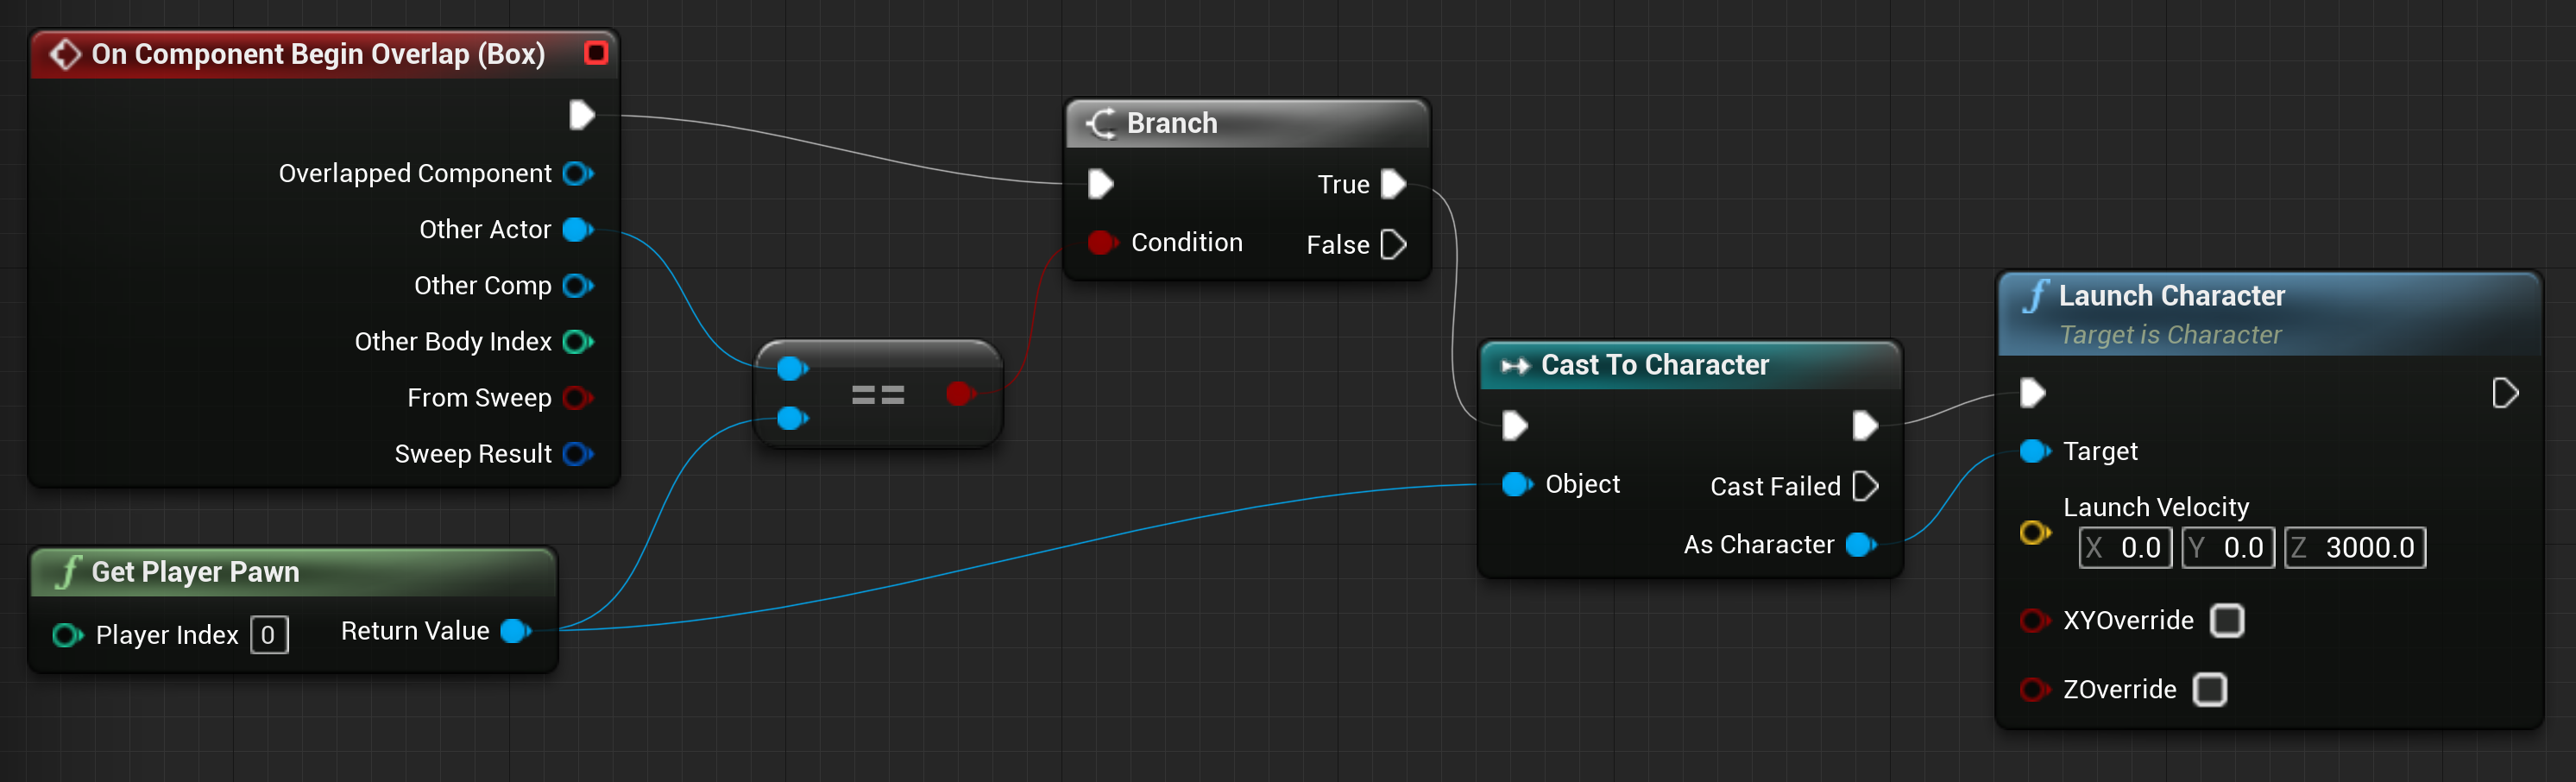
\includegraphics[width = 0.7\textwidth]{Imagenes/Blueprints.png}
	\caption{Blueprints en Unreal Engine}
	\label{fig:BluePrints_Figure}
\end{figure}

Además, Unreal Engine incluye un conjunto de herramientas preconfiguradas que facilitan el desarrollo, como sistemas de animación, iluminación, renderizado de alta calidad y físicas avanzadas. Gracias a estas características, cualquier usuario puede desarrollar videojuegos en 2D y 3D de manera accesible y rápida, sin necesidad de aprender un lenguaje de programación tradicional.

Si se compara con otros motores como Unity, Unreal Engine destaca por su calidad gráfica y su sistema visual más robusto. Mientras que en Unity se requiere programación para acceder a ciertas funciones avanzadas, en Unreal es posible construir mecánicas complejas únicamente con Blueprints. Esto lo convierte en una opción ideal para desarrolladores novatos que buscan facilidad de uso sin sacrificar potencia y flexibilidad.

Un punto negativo de Unreal Engine con respecto a Unity es la necesidad de recursos hardware que tiene para poder usarlo sin ningún tipo de ralentizaciones ni crasheos fortuitos, necesitando equipos muy potentes para que el desarrollo sea ameno o utilizar versiones anteriores de Unreal Engine.

Gracias a los Blueprints, cualquier persona puede diseñar enemigos, implementar IA, construir niveles interactivos y desarrollar mecánicas de juego avanzadas sin tocar código. 
\subsection{Godot}

Godot\footnote{\url{https://godotengine.org/}}, desarrollado por Juan Linietsky y Arenanet, es un motor de videojuegos de código abierto que ha ganado popularidad por su accesibilidad, flexibilidad y sencillez. Ofrece una plataforma poderosa para desarrollar videojuegos tanto en 2D como en 3D, y uno de sus mayores atractivos es que está diseñado para ser fácil de usar sin necesidad de tener conocimientos avanzados de programación.

A diferencia de otros motores como Unreal Engine o Unity, Godot permite el desarrollo de videojuegos con una interfaz intuitiva, pero también brinda herramientas más accesibles para aquellos que no desean escribir código. Su sistema de GDScript, un lenguaje propio diseñado específicamente para ser fácil de aprender y usar, facilita la creación de juegos sin necesidad de un conocimiento profundo de programación. GDScript es similar a Python (comparten sintaxis y tipado dinámico), lo que lo hace accesible y amigable para desarrolladores noveles.

Para aquellos que prefieren una experiencia más visual y menos enfocada en la programación, Godot incluye un sistema llamado \textit{VisualScript} (Figura \ref{fig:Godot_VisualScript_Figure}), un lenguaje visual basado en nodos que permite desarrollar mecánicas sin escribir código. Similar a los sistemas de programación visual en otros motores como Unreal Engine. Este sistema ha sido eliminado del núcleo de Godot a partir de la versión 4.0 del motor aunque en lanzamientos futuros VisualScript será re-implementado como una extensión\footnote{\url{https://docs.godotengine.org/es/3.5/tutorials/scripting/visual_script/index.html}}.

\begin{figure}[t]
	\centering
	\includegraphics[width = 0.7\textwidth]{Imagenes/VisualScriptGodot.pdf}
	\caption{Sistema VisualScript en Godot}
	\label{fig:Godot_VisualScript_Figure}
\end{figure}
Godot también destaca por ser un motor muy optimizado para el desarrollo de juegos en 2D, proporcionando una serie de herramientas específicas para este tipo de desarrollo, como un sistema de mallas 2D, animaciones, efectos y un conjunto de físicas dedicadas al mundo 2D. De esta manera, los desarrolladores pueden crear juegos con un rendimiento óptimo, incluso para dispositivos de baja gama, y con un flujo de trabajo ágil.

Comparado con otros motores como Unreal Engine o Unity, Godot se distingue por su flexibilidad y ligereza. Al no requierir licencias, lo convierte en una excelente opción para proyectos indie para estudios de pequeño y mediano tamaño. Aunque tradicionalmente ha sido asociado con el desarrollo indie como el roguelite \textit{Brotato}\footnote{\url{https://brotato.wiki.spellsandguns.com/Brotato_Wiki}} su adopcion ha crecido considerablemente siendo usado por titulod de mayor proyeccion como \textit{Marvel Snap}. También es especialmente potente para aquellos interesados en el desarrollo de juegos 2D, ya que ofrece herramientas específicamente diseñadas para este propósito, algo en lo que otros motores como Unity o Unreal Engine no se enfocan tanto.

La combinación de su accesibilidad y herramientas solventes hace que Godot permita a sus desarrolladores sin experiencia en programación crear juegos completos, desde mecánicas simples hasta sistemas complejos, sin necesidad de escribir código avanzado. Esta facilidad de uso, combinada con un motor robusto y libre, hace que Godot sea una opción popular para quienes buscan comenzar en el mundo del desarrollo de videojuegos o aquellos que desean una solución completamente gratuita y personalizable para sus proyectos.

Aunque Godot cuenta con grandes ventajas, cabe destacar que tanto Unity como Unreal son motores más establecidos en la industria, ya sea por la cantidad de assets, plugins o expansión de estos. 

\subsection{GameMaker}
\textit{GameMaker}\footnote{\url{https://gamemaker.io/en}} es un motor de videojuegos desarrollado por \textit{YoYo Games} que se especializa en la creación de juegos en 2D, aunque también cuenta con soporte limitado para gráficos en 3D. Su accesibilidad y facilidad de uso lo han convertido en una de las herramientas más populares entre desarrolladores indie, permitiendo la creación de títulos exitosos como \textit{Undertale}\footnote{\url{https://undertale.com}}, \textit{Hotline Miami}\footnote{\url{https://store.steampowered.com/app/219150/Hotline_Miami/}} o \textit{Katana ZERO}\footnote{\url{https://katanazero.com}}.\\

A diferencia de otros motores, GameMaker ofrece dos formas principales de desarrollo: un sistema de programación visual basado en eventos llamado \textit{Drag and Drop} y un lenguaje de scripting propio llamado \textit{GameMaker Language (GML)}. La opción de \textit{Drag and Drop} permite a los usuarios sin experiencia en programación crear juegos completos mediante una interfaz intuitiva de bloques gráficos (Figura \ref{fig:GameMaker_Figure}), mientras que \textit{GML} proporciona mayor control y flexibilidad a desarrolladores con conocimientos de programación.\\
\begin{figure}[t]
	\centering
	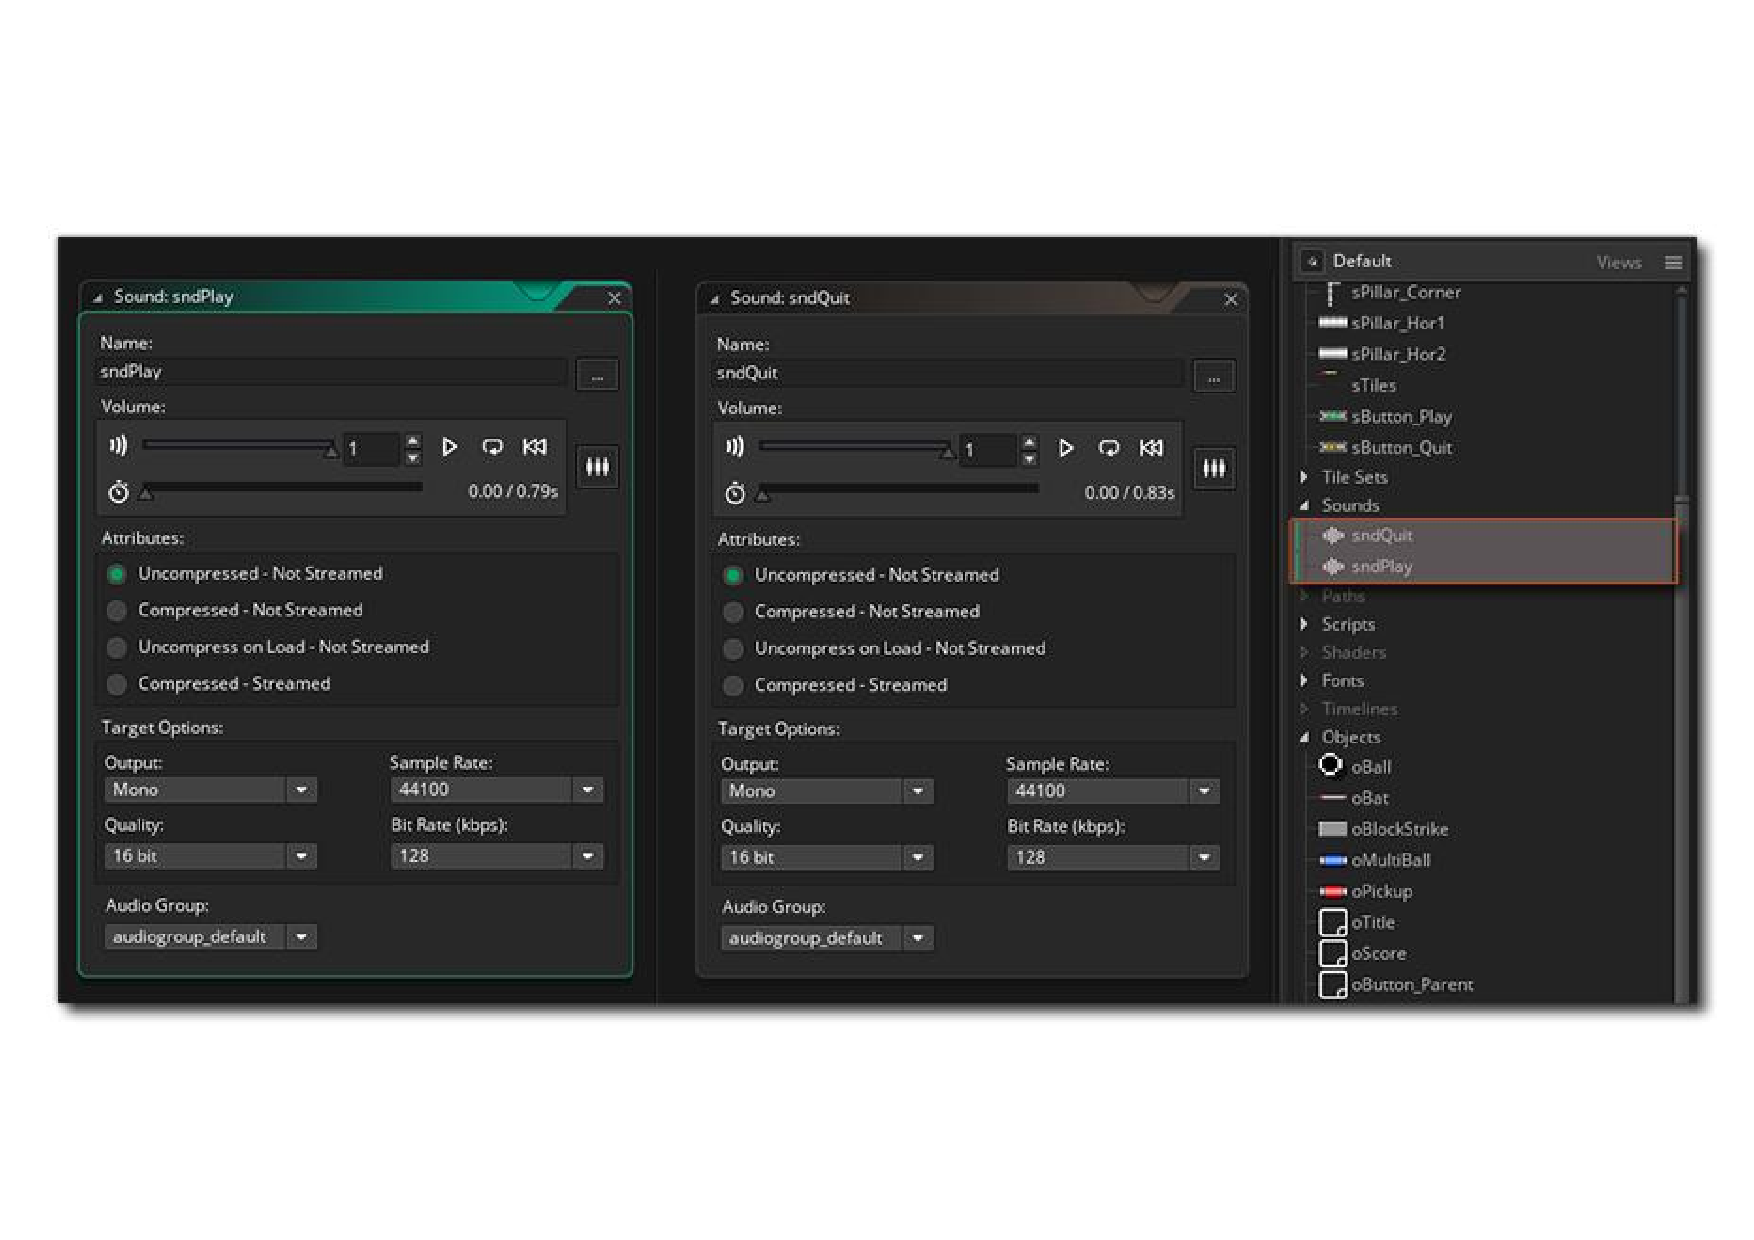
\includegraphics[width = 0.7\textwidth]{Imagenes/GameMaker.pdf}
	\caption{Drag and Drop en GameMaker}
	\label{fig:GameMaker_Figure}
\end{figure}

El sistema de \textit{Drag and Drop} funciona mediante la asignación de eventos y acciones a los objetos del juego. Por ejemplo, se pueden definir eventos como ``cuando el jugador presione una tecla'', seguido de una acción como "mover el personaje en una dirección". Esta metodología facilita la creación de juegos sin necesidad de escribir código, aunque también permite una transición fluida a \textit{GML} en caso de que el usuario desee más control sobre la lógica del juego.\\


Además de su sistema de scripting y su interfaz intuitiva, GameMaker incluye diversas herramientas preconfiguradas que agilizan el desarrollo, como un editor de sprites incorporado, un sistema de animación, un motor de colisiones y soporte para efectos visuales mediante \textit{shaders}. Gracias a estas características, cualquier usuario puede desarrollar videojuegos en 2D sin necesidad de aprender un lenguaje de programación desde cero.\\

Si se compara con otros motores como \textit{Unity}, GameMaker se destaca por su rapidez y facilidad de uso en proyectos en 2D. Mientras que en \textit{Unity} la configuración de un juego en 2D puede requerir una mayor curva de aprendizaje, GameMaker permite comenzar a desarrollar desde el primer momento con una interfaz optimizada para este tipo de juegos. Sin embargo, su soporte para gráficos en 3D es limitado en comparación con \textit{Unreal Engine} o \textit{Unity}, lo que lo hace menos adecuado para proyectos que requieran entornos tridimensionales complejos.\\

Un punto negativo de GameMaker con respecto a otros motores es que algunas funciones avanzadas, como la exportación a consolas o la personalización del motor, requieren licencias de pago, lo que puede representar una barrera para algunos desarrolladores. Sin embargo, su modelo de suscripción y la posibilidad de utilizar la versión gratuita para prototipado lo convierten en una opción accesible para quienes buscan una herramienta de desarrollo rápida y eficiente.\\

Gracias al sistema de \textit{Drag and Drop} y \textit{GML}, cualquier persona puede crear plataformas interactivas, implementar inteligencia artificial básica, desarrollar mecánicas de combate y programar juegos completos sin necesidad de utilizar motores más complejos.\\
\section{Conclusiones}

A lo largo del análisis, se han recopilado los aspectos positivos tanto de las herramientas como de los motores de videojuegos estudiados, con el objetivo de utilizarlos como referencia e inspiración en el desarrollo del proyecto. Este proyecto está diseñado específicamente para desarrolladores noveles, proporcionando una solución accesible y flexible para la creación de enemigos en videojuegos de plataformas 2D.\\

El proyecto consistirá en una serie de componentes modulares, que permitirán a los desarrolladores generar enemigos de manera sencilla y eficiente. Estos componentes estarán diseñados para facilitar la implementación de comportamientos básicos sin requerir un conocimiento profundo de programación o inteligencia artificial. Además, la arquitectura del sistema garantizará que la herramienta sea escalable, permitiendo la incorporación de nuevos componentes en el futuro para ampliar su funcionalidad según las necesidades del usuario.\\

En cuanto a técnicas de modelado analizadas, se han identificado varias características destacables que servirán de referencia para el diseño del proyecto. PlayMaker sobresale por su sistema de scripting visual, el cual simplifica la representación y modificación de máquinas de estado finitas (FSM), haciendo que la creación de comportamientos sea más intuitiva. Por otro lado, Unity ofrece un inspector versátil y de fácil entendimiento, lo que facilita la configuración y manipulación de objetos en el entorno de desarrollo.\\

En conclusión, el desarrollo de esta herramienta busca simplificar la creación de enemigos en videojuegos 2D, brindando a los desarrolladores principiantes una forma accesible de implementar inteligencia artificial básica. Al integrar los aspectos positivos de las herramientas y motores estudiados, se espera proporcionar una solución flexible, escalable y fácil de usar, fomentando la creatividad y el aprendizaje en el desarrollo de videojuegos.\\